\documentclass{scrartcl}
\usepackage[utf8]{inputenc} % Unicode support (Umlauts etc.)
\usepackage{hyperref} % Add a link to your document
\usepackage{graphicx} % Add pictures to your document
\usepackage{listings} % Source code formatting and highlighting
\usepackage[top=75px, bottom=75px, left=85px, right=85px]{geometry} % Change page borders
\usepackage{graphicx}
\usepackage{mathtools}


\begin{document}

\title{Computational Intelligence:
\\Report assignment 3}
\date{\today{}}

\author{
    \begin{tabular}{l r}
    	\\Tjitte de Jong - 4172930
	\\Boris Mulder - 4100794
        \\Max Spanoghe - 4331834
            \end{tabular}
  }
  
\maketitle \thispagestyle{empty} \pagebreak
  
\section*{ANT PREPARATION: OBSERVE THE PROBLEM}
  Here we will answer the questions about the observation of the problem.
  
\subsection*{1.}
First of all it could be possible that the ant is in a very big room. This would be difficult because it is hard to find the exit and the ant can make an unnecessary turns which can lead to a very long path.
Secondly, it could happen that the ant gets in a dead end and needs to go back all the way to a previous choice point.

\subsection*{2.}
The ants drop Pheromones to let the other ants know the popularity of a certain path. The amount of pheromone dropped is dependent on how long the path is that he took. The equation which determines the amount of pheromones par path is: \\
$Pheromone_on_link_i = \frac{n}{Path length}$
The parameter n is the estimated pathlength.

\subsection*{3.}
 The evaporation of a link i is is actually the Pheromones that are getting away from that link. For example:\\
 evaporation constant $\alpha$ = 0.1;\\
 Pheromones on link in iteration i = p ;\\
 Then \\
 Pheromones on link in next iteration = (1-$\alpha$)*p;\\
 The evaporation is very handy to get a more quick convergence to a certain path. If a path it not chosen the links on that path get less pheromones after each iteration. In this way, the chances that ants take a path that is not very popular decreases much faster. Each iteration the pheromones go down relatively because they don't take the path, but also because of the evaporation.
 \pagebreak
 \section*{IMPLEMENTING SWARM INTELLIGENCE}
 Here we will answer the questions about the actual implementation.
 
 \subsection*{4.}
 The following parameters are used in the basic version of our system:\\
 $ iterations = 30; $\\
 $ ants = 3; $ \\
 $ pher = estimate of route length; $\\
 $ evaporation constant = 0.9;we want fast convergence) $\\ 
converge criterion is when the first ant in 5 iterations take the same path.\\
pseudo-code:\\
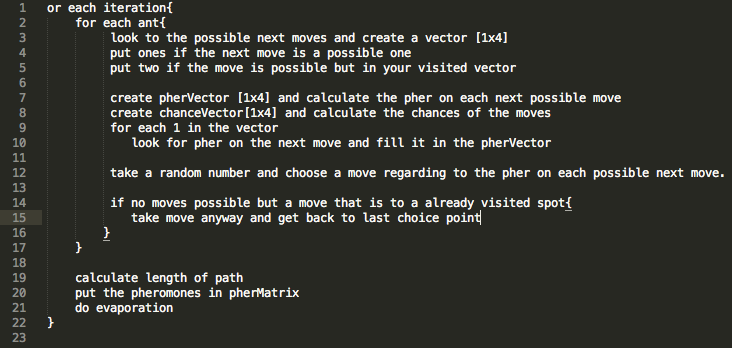
\includegraphics[width=1\textwidth]{pseudo.PNG}

\pagebreak
\section{UPGRADING YOUR ANTS WITH INTELLIGENCE}
Here we will answer the questions about how to upgrade the intelligence of the ants.

\subsection*{5.}
Especially for the big rooms we have found a better solution than the normal maze solving algorithm we had before. The way it works is pretty good and still easy enough to implement quickly. If the ant enters a big room we do a check. If the ant has four possible next moves he will do this as long as he has 4 next possible moves:\par
take a direction just based on the normal solution and forbid him to take the opposite direction again.
In this way, he will move but never have loops in a big room. It stops when he hits a wall, bounce and will do it again eventually. This method prevent the ant of doing stupid loops in a big room. For example, if you are in a big room and you cannot see the actual walls. What one would do is start walking until he sees a wall, but never move back until you have found one, since you know there is nothing there but open space. Once you see a wall and you see there is no exit, you will bounce and start walking in the other direction again or just follow the walls. This is actually what this algorithm does so it actually works like a real person would solve the maze big rooms.

\section*{PARAMETER OPTIMIZATION}
Here we will answer the questions about the optimization of the parameters.
\subsection*{6.}
\subsection*{7.}




















\pagebreak
\section*{PART 2: THE TRAVELING ROBOT PROBLEM}
\section*{Problem analysis}
Here we will answer the questions about the TSP problem.

\subsection*{8.}
A traveling salesman problem is defined as following. A trader needs to find a route in which he makes sure that he starts at one city, travels to all other cities once and then come back. Each connection between to cities has a specified length. You can obviously do this in many many ways. The actual problem is thus to find the shortest route to go to all cities and then come back to the first one.
If you have 3 cities you can either start in 1/2/3. Then you can have following routes to take:\\
$1=>2=>3=>1$\\
$1=>3=>2=>1$\\
$2=>1=>3=>2$\\
...
You cannot calculate the total length of each path when the number of cities (nodes) gets high since the number of possible routes then increases at an enormously high rate. ( $nodes! = nodes*(nodes-1)*(nodes-2)....*1$)

\subsection*{9.}
The difference in this problem lies in the fact that there is a starting point and also and specified end point. So actually there is a smaller TSP problem between the point except the first and the last point since they are fixed.

\subsection*{10.}
They are made for searching through a vast open solution space and because they are able to find decent solutions by their techniques of using a fitness function and then change the solutions in such a way that it will make the error lower so you can find better solutions as long as you iterate. This is what you want to do with this problem since brute force will never work out on large numbers of nodes. Therefore they are very handy in this kind of situations.

\subsection*{11.}
The genes represent the node to go to. A chromosome in a TSP with 5 nodes \\(excluding the begin point 1 and end point 7) would look like this: \\
\begin{tabular}{ | l | l | l | l | l | l | l |}
  \hline			
  1 & 5 & 2 & 4 & 6 & 3 & 7  \\
  \hline  
\end{tabular}\\
One number is one gene and the whole sequence is one chromosome. Each chromosome represents a route from 1 to 7 with different sequence of the points in the list.
\\
Our group didn't encode the chromosomes into a encoded chromosome because it is not actually needed since the sequence which are solutions are actually already in the format of a chromosome.

\subsection*{12.}
Our group used the following fitness function:\\
$fitness = 1/pathlength$

\subsection*{13.}
Our group used the roulette wheel selection method. This means that first the ratios of each chromosome in the populations gets calculated as following: \\
$ratio = fitness / totalFitness$\\
The good/best paths get a higher chance in this ratio calculation. Then a random number is chosen and there is checked in which interval it lies. Based on this, one of the chromosomes in the first population is chosen for the new population.

\subsection*{14.}
Our group both implemented the mutations and the cross-over. For the cross over there is made a selection of two chromosomes in the parent population and they produce a new permutation of the numbers by using a fairly common method:\\
\\
'Single point crossover - one crossover point is selected, till this point the permutation is copied from the first parent, then the second parent is scanned and if the number is not yet in the offspring it is added
Note: there are more ways how to produce the rest after crossover point.'\\
See source: http://www.obitko.com/tutorials/genetic-algorithms/crossover-mutation.php\\
\\
For mutations we just made sure that two points get swapped (except the first and the last point since they are still fixed). In this way you make sure that the there are no double numbers in the sequence and that there are numbers lacking.

\subsection*{15.}
Because we make use of a smarter mutation as mentioned above there will never be two numbers in the chromosome that are the same. They will all be unique and the first and last one will always be fixed.

\subsection*{16.}
We prevent local minima by using these mutations. They will make sure that sometimes the route is changed in such a way that for a moment it could be that the length of the route is worse but after a while maybe a better route can be found by changing that one. Also cross over does the same thing but in a different way.

\subsection*{17.}
Our group used elitism indeed. But not in the formal way. The formal way is to make sure the best route always get selected from the parent population to be part of the child population. What our group did instead is making the fitness function not linear but squared. In this way the worse the path is, the less chance it gets to be selected. We tried out both but found out that this method works faster.




\pagebreak
\begin{figure}[h!]
  \centering
    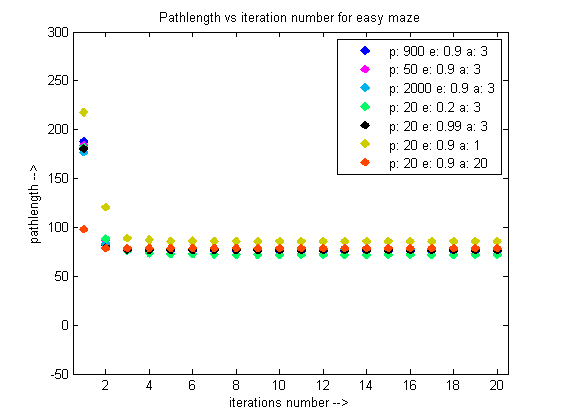
\includegraphics[width=0.5\textwidth]{Plot_easy.PNG}
      \caption{Plot of different sets of parameters and their convergence for the easy maze.}
    \label{figure1}
\end{figure}

\begin{figure}[h!]
  \centering
    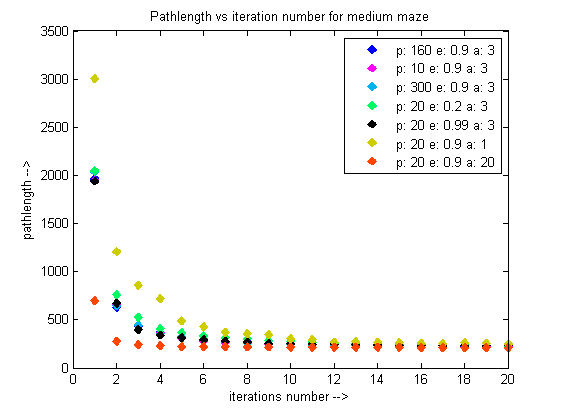
\includegraphics[width=0.5\textwidth]{Plot_medium.PNG}
    \caption{Plot of different sets of parameters and their convergence for the medium maze.}
    \label{fiure2}
\end{figure}

\begin{figure}[h!]
  \centering
    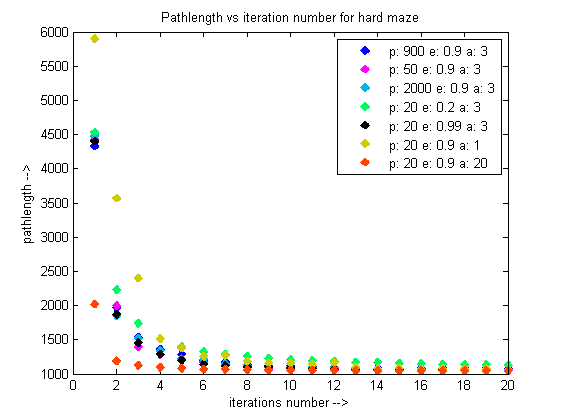
\includegraphics[width=0.5\textwidth]{Plot_hard.PNG}
      \caption{Plot of different sets of parameters and their convergence for the hard maze.}
    \label{figure3}
\end{figure}





 
 
 
 	
		 
		 
		
 
\end{document}